% Drawing 73/01-16 -- folder 73, batch 01, archive page 17 (PDF page 18).
% Transcription: en bas, sous une ligne ondulée : à gauche deux vecteurs qui se suivent, $u$ montant vers la droite puis $v$ descendant ; à droite un pentagone avec ses cinq diagonales, un coin hachuré.
% Kind: two consecutive vectors u, v; pentagon with all its diagonals. Method 2 (schematic redraw from the facsimile). Status: ok.
% Notes: As on the page: the wavy line across the page; the vector u (slightly curved) and the vector v from its tip, each with its arrowhead and letter; the pentagon, its five sides and five diagonals between the same five vertices; four short hatching strokes in the upper left corner triangle. Left out: the struck formula under the vectors. Redrawn 2026-11-12 (issue 128): to check again.
% Coordinates: 1 unit = 1 mm = 1/100 of the crop width (bbox in page fractions: [0.1, 0.74, 0.62, 0.89]).
% Redrawn by Claude (claude-fable-5-2), issue #128, 2026-11-12; not checked by a human; not compiled (no TeX in the session).
% Rights: reproduces part of the work -- behind RENDER_TRANSCRIPTS, never published by itself.
\documentclass[tikz,border=3pt]{standalone}
\usepackage{amsmath,amssymb}
\usetikzlibrary{patterns,arrows.meta}
\tikzset{pencil/.style={black!45}, struck/.style={black!35}, mpt/.style={circle,draw,inner sep=1.3pt}, pt/.style={circle,fill,inner sep=0.9pt}, opt/.style={circle,draw,fill=white,inner sep=1.1pt}}
\begin{document}
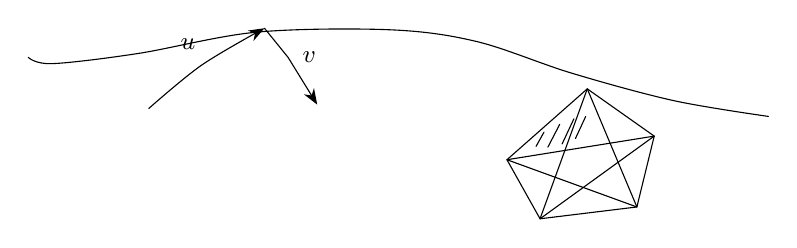
\begin{tikzpicture}[x=1mm,y=1mm,line cap=round,line join=round,font=\scriptsize]
\draw plot[smooth, tension=0.55] coordinates {(6,-12) (9,-12.8) (20,-11.5) (35,-8.8) (52,-8.5) (63,-10) (75,-14) (88,-17.5) (100,-19.5)};
\draw[-{Stealth[length=2mm]}] plot[smooth, tension=0.55] coordinates {(21.3,-18.5) (28,-13) (36,-8.3)};
\draw[-{Stealth[length=2mm]}] (36,-8.3) -- (39,-12) -- (42.7,-18);
\node[inner sep=1pt] at (26.3,-10.3) {\small $u$};
\node[inner sep=1pt] at (41.7,-12) {\small $v$};
\draw (66.8,-25) -- (77,-16) -- (85.5,-22) -- (83.3,-31) -- (71,-32.5) -- cycle;
\draw (66.8,-25) -- (85.5,-22);
\draw (77,-16) -- (83.3,-31);
\draw (85.5,-22) -- (71,-32.5);
\draw (83.3,-31) -- (66.8,-25);
\draw (71,-32.5) -- (77,-16);
\draw (70.5,-23.3) -- (71.5,-21.5);
\draw (72,-23.4) -- (73.5,-20.5);
\draw (73.8,-23) -- (75.3,-19.8);
\draw (75.5,-22.3) -- (76.8,-19.5);
\end{tikzpicture}
\end{document}
